\documentclass{beamer}
\usefonttheme[onlymath]{serif}
\usepackage{amsmath}
\usepackage{amsfonts}
\usepackage[export]{adjustbox}
\usepackage[utf8]{inputenc}
\usepackage{tikz} 
\usetikzlibrary{bayesnet}

% definitions
\def\H{\mathcal{H}}
\def\X{\mathbf{X}}
\def\w{\mathbf{w}}
\def\W{\mathbf{W}}
\def\const{\mathrm{const}}
\def\Var{\mathrm{Var}}
\def\tr{\mathrm{tr}}
\def\T{\top}
\def\U{\mathbf{U}}
\def\S{\mathbf{S}}
\def\V{\mathbf{V}}
\def\N{\mathcal{N}}
\def\E{\mathbb{E}}
\newcommand{\argmin}{\mathop{\mathrm{argmin}}}
\newcommand{\argmax}{\mathop{\mathrm{argmax}}}
\newcommand{\minimize}{\mathop{\mathrm{minimize}}}
\newcommand{\maximize}{\mathop{\mathrm{maximize}}}
\newcommand{\st}{\mathop{\mathrm{subject\,\,to}}}

%Information to be included in the title page:
\usecolortheme{seahorse}
\title{Dynamic Model}
\author{Thomas Bayes}
\institute{
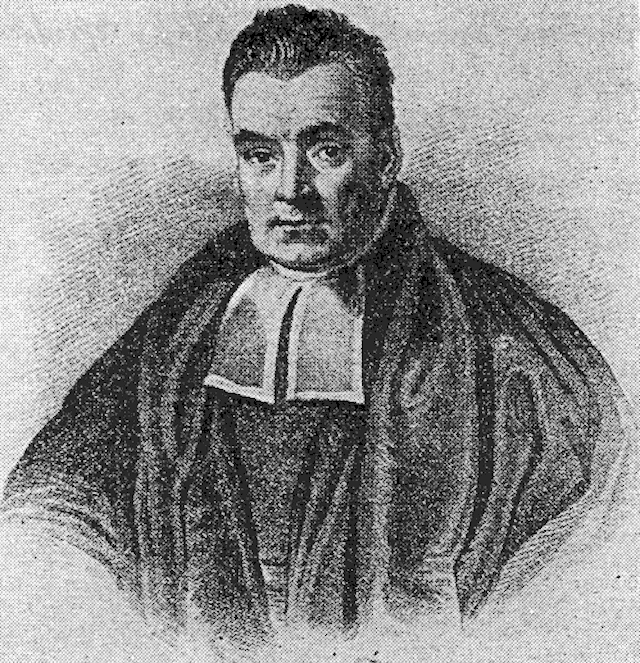
\includegraphics[height=.3\textheight]{../bayes.png}%
}
\date{\today}

    
    
\begin{document}
    
\frame{\titlepage}

\begin{frame}{Introduction}
We are going to introduce the state space models and their corresponding algorithms, \textbf{Kalman Filter} and \textbf{Particle Filter}.

\end{frame}
\begin{frame}{State Space Model}

\begin{figure}[H]
    \centering
    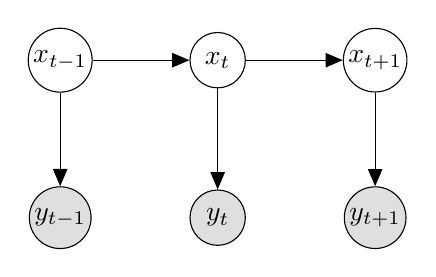
\begin{tikzpicture}
      % Nodes
      % parameters and data
      \node[latent] (X1) {$x_{t-1}$};
      \node[latent,xshift=2cm] (X2) {$x_{t}$};
      \node[latent,xshift=4cm] (X3) {$x_{t+1}$};
      \node[obs, yshift=-2cm] (O1) {$y_{t-1}$};
      \node[obs, yshift=-2cm, xshift=2cm] (O2) {$y_t$};
      \node[obs, yshift=-2cm, xshift=4cm] (O3) {$y_{t+1}$};
      \edge{X1}{O1}
      \edge{X2}{O2}
      \edge{X3}{O3}
      \edge{X1}{X2}
      \edge{X2}{X3} 

    \end{tikzpicture}
    \end{figure}
In state space model, we have state variable sequence $x_1, \dots, x_t$ and observed variables sequence $y_1, \dots, y_t$. State variables means the hidden state behind the world. 
We now have the representation of state space model, now assume we know the all parameters of our model. What if we want to do inference of the model? In such model, we are particularly interested in two tasks.
\begin{itemize}
\item Prediction $$p(y_t | x_{1:t})$$
\item Update $$p(y_t | x_{1 : t-1})$$
\end{itemize}
\end{frame}

\begin{frame}{Inference of Kalman Filter}
In Kalman Filter, we assume that 
$$p(x_t | x_{t-1}) \sim \mathcal{N} (A x_{t-1} + B, Q)$$
and 
$$p(y_t | x_t) \sim \mathcal{N}(Hx_t, R)$$
So we say that Kalman Filter is a linear model. In inference task, we assume that we already know all the parameters of the model, $A, B, Q, H,R$, and based on the observation $y_{1:t}$, we infer the probability distribution of the underlying state $x_t$. Here note that we can't use information from future, $y_{t+1}$ to infer the underlying state $x_t$.
\end{frame}

\begin{frame}{From Update to Prediction}
If 
$$p(x) \sim \N(x | \mu, \Sigma) \qquad p(y|x) \sim \N(y | Ax + b, L)$$
we have 
$$p(y)=\int_x p(y | x) p(x) dx \sim \N(y | A\mu + b, L + A\Sigma A^\top)$$
So for prediction task, we have
\begin{align*}
p(x_t | y_{1 : t-1}) & \sim \N(\bar{\mu}_t, \bar{\Sigma}_t) = \int_{x_{t-1}}p(x_t | x_{t-1})p(x_{t-1}|y_{1:t-1}) dx_{t-1} \\
& = \int_{x_{t-1}} \N(x_t | Ax_{t-1} + B, Q) \N(x_{t-1} | \hat{\mu}_{t-1}, \hat{\Sigma}_{t-1}) \\
& = \N(x_t | A \hat{\mu}_{t-1} + B, A\hat{\Sigma}_{t-1}A^\top + Q)
\end{align*}
So we use the parameters $\hat{\mu}_{t-1}$ and $\hat{\Sigma}_{t-1}$ of previous \textbf{update} to infer the \textbf{prediction} of state $t$.
\end{frame}

\begin{frame}[allowframebreaks]{From Prediction to Update}
For this task, we use an alternative approach, by taking advantage of property of Gaussian distribution
$$x_{t-1} | y_{1:t-1} \sim \N(\E[x_{t-1}], \hat{\Sigma}_{t-1})$$
We attempt to write $\Delta x_t$ and $\Delta y_t$ in term of $\Delta x_{t-1}$
$$x_t = Ax_{t-1} + w_t \quad w_t \sim \N(0, Q)$$
And we get 
\begin{align*}
x_t|y_{1:t-1} & = A(\Delta x_{t-1} + \E[x_{t-1}]) + w_t \\
& = A\E[x_{t-1}] + B + \underbrace{A\Delta x_{t-1} + w_t}_{\Delta x_t | y_{1:t-1}}
\end{align*}

\framebreak

For $y_t$,
$$y_t = Hx_{t-1} + v_t \quad v_t \sim \N(0, R)$$
\begin{align*}
y_t|y_{1:t-1} & = H(A\E[x_{t-1}] + B + A\Delta x_{t-1} + w_t) + v_t \\
& = HA\E[x_{t-1}] + HB + \underbrace{HA\Delta x_{t-1} + Hw_t + v_t}_{\Delta y_t | y_{1 : t-1}}
\end{align*}

So we have the expression of $x_t|y_{1:t-1}$ and $ y_t | y_{1 : t-1}$.
And we are aiming to get the expression of $x_t | y_{1:t}$.
For Gaussian distribution, we have the property
$$p(u) = \N(\mu_u, \Sigma_{uu}) \qquad p(v) = \N(\mu_v, \Sigma_{vv})$$
and 
$$p(u | v) = \N(\mu_u + \Sigma_{uv} \Sigma_{vv}^{-1}(v - \mu_v), \Sigma_{uu} - \Sigma_{uv}\Sigma_{vv}^{-1}\Sigma_{vu})$$

\framebreak 
Imagine $p(u) = p(x_t | y_{1 : t-1})$ and $p(v) = p(y_t | y_{1 : t-1})$, so $p(u |v) = p(x_t | y_{1:t})$.
Now we just need to calculate $\Sigma_{uu}, \Sigma_{uv}, \Sigma_{vv}$.

$$\Sigma_{uu} = A \hat{\Sigma}_{t-1} A^\top + Q = \bar{\Sigma}_t$$
$$\Sigma_{vv} = HA \hat{\Sigma}_{t-1}A^\top H^\top + HQ H^\top + R = H \bar{\Sigma}_t H^\top +R$$
$$\Sigma_{uv} = H(A\hat{\Sigma}_{t-1}A^\top + Q) = H\bar{\Sigma}_t$$
We substitute these into the following and will get the result.
$$p(u | v) = \N(\mu_u + \Sigma_{uv} \Sigma_{vv}^{-1}(v - \mu_v), \Sigma_{uu} - \Sigma_{uv}\Sigma_{vv}^{-1}\Sigma_{vu})$$
So we have used $\bar{\Sigma}_t, \hat{\mu}_t$ and parameters to express $p(x_t | y_{1:t})$.
So from the update parameter $p(x_{t-1} | y_{1:t-1}) \sim \N(\hat{\mu}_{t-1}, \hat{\Sigma}_{t-1})$ we get the prediction parameter of $p(x_t | y_{1:t-1})$. And from parameter of prediction $\bar{\Sigma}_t, \hat{\mu}_t$, we can get the paramter of update.

\framebreak 

So the pipeline is like 
$$\text{prediction}_t \longrightarrow \text{update}_t \longrightarrow \text{prediction}_{t+1}$$

\end{frame}

\begin{frame}[allowframebreaks]{Learning Kalman Filter}


\end{frame}



\end{document}